\selectlanguage{spanish}

\renewcommand{\articuloidiomaxml}{es}
\renewcommand{\articulotitulo}{El desarrollo agropecuario argentino en la segunda posguerra}
\renewcommand{\articuloautores}{Marcelo Rougier}
\renewcommand{\articulodoi}{10.56503/H-Industria/n.37(19)/3473}
\renewcommand{\articulotipo}{ARTÍCULO DE INVESTIGACIÓN}
\renewcommand{\articulorevista}{H-industria}
\renewcommand{\articuloissne}{1851-703X}
\renewcommand{\articulovolumen}{01}
\renewcommand{\articulonumero}{01}
\renewcommand{\articulofecha}{ 2026}
\renewcommand{\articulopagina}{23}

\setcounter{page}{23}
\thispagestyle{firstpage}

% --- TÍTULO A ANCHO COMPLETO ---
\noindent\begin{minipage}[t]{\dimexpr\textwidth+\marginparsep+\marginparwidth\relax}%
{\sffamily\bfseries\Large\articulotitulo\par}%
\end{minipage}\par
\vspace{3mm}%
\renewcommand{\articulotitulotrans}{Argentine Agricultural Development in the Second Postwar Period}
\noindent\begin{minipage}[t]{\dimexpr\textwidth+\marginparsep+\marginparwidth\relax}%
{\sffamily\itshape\normalsize\articulotitulotrans\par}%
\end{minipage}\par
\vspace{4mm}%

% --- BLOQUE LATERAL DE METADATOS ---
\begin{textblock*}{68mm}(\gbbloquex,92mm)
{\setlength{\leftskip}{0pt}\setlength{\parindent}{0pt}%
\noindent\begin{minipage}[t]{68mm}
\sffamily\small\setlength{\parskip}{1pt}
{\bfseries\color{azulrevista}Marcelo Rougier}\par
{\scriptsize\texttt{\href{https://orcid.org/0009-0002-5273-5191}{https://orcid.org/0009-0002-5273-5191}}}\par
Consejo Nacional de Investigaciones Científicas y Técnicas\par
\vspace{6pt}
{\bfseries\color{azulrevista!70}Derechos de autor\'ia:}\par
\textcopyright\ 2026 Rougier, M. Publicado por H-industria. Se permite el uso, distribución y reproducción sin fines comerciales, siempre que se cite la obra original y las obras derivadas se distribuyan bajo la misma licencia. (\href{https://creativecommons.org/licenses/by-nc-sa/4.0/}{https://creativecommons.org/licenses/by-nc-sa/4.0/})\par\vspace{6pt}
{\bfseries\color{azulrevista!70}Publicación:} 2026, vol.~01, n\'um.~01, pp.~23--43\par\vspace{6pt}
{\bfseries\color{azulrevista!70}URL:} {\scriptsize\texttt{\href{https://www.edicionesimagomundi.com/}{https://www.edicionesimagomundi.com/}}}\par\vspace{6pt}
{\bfseries\color{azulrevista!70}DOI:} {\scriptsize\texttt{\href{https://doi.org/10.56503/H-Industria/n.37(19)/3473}{10.56503/H-Industria/n.37(19)/3473}}}\par\vspace{6pt}
{\bfseries\color{azulrevista!70}Licencia:} CC BY-NC-SA 4.0\par
{\scriptsize\texttt{\href{https://creativecommons.org/licenses/by-nc-sa/4.0/}{https://creativecommons.org/licenses/by-nc-sa/4.0/}}}\par
\vspace{6pt}
{\bfseries\color{azulrevista!70}Fechas}\par\vspace{2pt}
Recibido: 05/01/2026\par
Aceptado: 19/01/2026\par
Online: 25/02/2026\par
\vspace{6pt}
\vspace{6pt}
{\bfseries\color{azulrevista!70}Compartir:}\par\vspace{3pt}
{\large
\href{https://www.linkedin.com/sharing/share-offsite/?url=https%3A%2F%2Fwww.edicionesimagomundi.com%2F}{\textcolor{azulrevista}{\faLinkedin}}~
\href{https://twitter.com/intent/tweet?url=https%3A%2F%2Fwww.edicionesimagomundi.com%2F&text=El%20desarrollo%20agropecuario%20argentino%20en%20la%20segunda%20posguerra}{\textcolor{azulrevista}{\faTwitter}}~
\href{https://www.researchgate.net/search?q=El%20desarrollo%20agropecuario%20argentino%20en%20la%20segunda%20posguerra}{\textcolor{azulrevista}{\faResearchgate}}~
\href{https://www.reddit.com/submit?url=https%3A%2F%2Fwww.edicionesimagomundi.com%2F&title=El%20desarrollo%20agropecuario%20argentino%20en%20la%20segunda%20posguerra}{\textcolor{azulrevista}{\faReddit}}~
\href{mailto:?subject=El%20desarrollo%20agropecuario%20argentino%20en%20la%20segunda%20posguerra&body=https%3A%2F%2Fwww.edicionesimagomundi.com%2F}{\textcolor{azulrevista}{\faEnvelope}}~
\href{https://www.facebook.com/sharer/sharer.php?u=https%3A%2F%2Fwww.edicionesimagomundi.com%2F}{\textcolor{azulrevista}{\faFacebook}}~
\href{https://wa.me/?text=https%3A%2F%2Fwww.edicionesimagomundi.com%2F}{\textcolor{azulrevista}{\faWhatsapp}}~
\href{https://t.me/share/url?url=https%3A%2F%2Fwww.edicionesimagomundi.com%2F&text=El%20desarrollo%20agropecuario%20argentino%20en%20la%20segunda%20posguerra}{\textcolor{azulrevista}{\faTelegram}}
}\par
\end{minipage}%
}% FIN GRUPO leftskip
\end{textblock*}


\begin{tcolorbox}[colback=brown!8!white,colframe=brown!8!white,boxrule=0pt,arc=2pt,left=4pt,right=4pt,top=3pt,bottom=3pt,before skip=4pt,after skip=4pt]
\begin{otherlanguage}{spanish}
\sffamily\small \textbf{Resumen:} El dossier analiza el desarrollo agropecuario argentino entre 1950 y 1970, en el marco de los debates sobre desarrollo e industrialización. Examina políticas públicas, crédito, tecnología y agroindustrias regionales, destacando tensiones, continuidades y su impacto social, productivo y ambiental.
\par\smallskip\noindent\textbf{Palabras clave:} Desarrollo agropecuario, Industrialización, Políticas públicas, Agroindustria, Tecnología agraria, Argentina
\end{otherlanguage}
\end{tcolorbox}

\begin{tcolorbox}[colback=brown!8!white,colframe=brown!8!white,boxrule=0pt,arc=2pt,left=4pt,right=4pt,top=3pt,bottom=3pt,before skip=4pt,after skip=4pt]
\begin{otherlanguage}{english}
\sffamily\small \textbf{Abstract:} This dossier examines Argentine agricultural development from the 1950s to the 1970s within debates on development and industrialization. It explores public policies, credit, technology, and regional agribusiness, highlighting tensions, continuities, and their social, productive, and environmental impact.
\par\smallskip\noindent\textbf{Keywords:} Agricultural development, Industrialization, Public policy, Agribusiness, Agricultural technology, Argentina
\end{otherlanguage}
\end{tcolorbox}

\begin{tcolorbox}[colback=brown!8!white,colframe=brown!8!white,boxrule=0pt,arc=2pt,left=4pt,right=4pt,top=3pt,bottom=3pt,before skip=4pt,after skip=4pt]
\begin{otherlanguage}{portuguese}
\sffamily\small \textbf{Resumo:} O dossiê analisa o desenvolvimento agropecuário argentino entre as décadas de 1950 e 1970, no contexto dos debates sobre desenvolvimento e industrialização. Examina políticas públicas, crédito, tecnologia e agroindústrias regionais, destacando tensões, continuidades e impactos sociais, produtivos e ambientais.
\par\smallskip\noindent\textbf{Palavras-chave:} Desenvolvimento agropecuário, Industrialização, Políticas públicas, Agroindústria, Tecnologia agrícola, Argentina
\end{otherlanguage}
\end{tcolorbox}

\bigskip
\noindent\rule{\linewidth}{0.4pt}
\bigskip


\epigraph{Contener los reclamos populares mediante reformas orientadas a mejorar las condiciones de vida.

}{Francis Bacon}

Finalizada la Segunda Guerra Mundial, en una coyuntura marcada por los procesos de des­colonización en Asia y África, los movimientos de liberación nacional y las revoluciones so­cialistas, surgieron diversas teorías y debates en torno a las vías de desarrollo que debían seguir los países considerados “atrasados” para alcanzar los estándares económico-sociales de las potencias. Paralelamente, el temor de las clases dominantes ante el avance del comu­nismo y las transformaciones sociales que se evidenciaban en la región se tradujo en una serie de iniciativas destinadas a contener los reclamos populares mediante reformas orientadas a mejorar las condiciones de vida.


\begin{quote}
A través del análisis e integración de fuentes oficiales y de las publicaciones de las principales entidades y corpo­raciones del sector, logran reconstruir la conflictividad del período e identificar el impacto de dichos conflictos en la dinámica política de esos años.

\end{quote}


\begin{figure}[!ht]
\centering
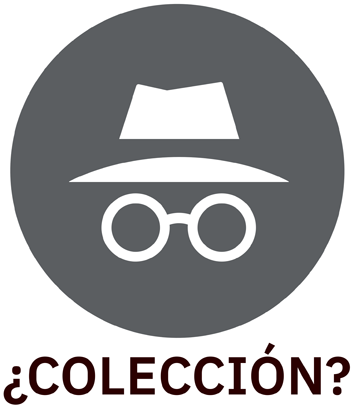
\includegraphics[width=\linewidth]{../media/desconocido.png}
\captionof{figure}{descripción de la imagen}
\label{fig-1}
\label{fig-1}
\vspace{\intextsep}
\end{figure}


\begin{adjustwidth}{0pt}{-\dimexpr\marginparsep+\marginparwidth\relax}%
\centering

\includegraphics[width=\linewidth]{../media/imagen3.png}
\captionof{figure}{descripción de la imagen}
\label{fig-2}
\label{fig-2}
\vspace{\intextsep}
\end{adjustwidth}

Las nuevas teorías del desarrollo situaron a la producción manufacturera en el centro de sus preocupaciones: era imperioso modificar la estructura productiva a través de la trans­ferencia de recursos desde sectores como la agricultura. Para la mayoría de los intelectuales y profesionales que participaron del debate, esta era la “llave” para el despegue. En América Latina, aunque el impulso a un crecimiento industrial integrado ocupó un lugar destacado en la agenda pública, las problemáticas agrarias y las discusiones sobre la propiedad de la tierra también adquirieron gran relevancia. Por cierto, muchos intelectuales latinoamericanos –en­tre los que se contaban los cepalinos– cuestionaron la orientación “hacia afuera” de las eco­nomías del subcontinente y comenzaron a legitimar una nueva, para lo que resultaba rele­vante analizar la producción agraria y su rol como proveedora de divisas en un contexto en el que, desde la Comisión Económica para América Latina, se defendía la industrialización como un medio para alcanzar el desarrollo \cite{1254-FAJARDO2025}.


\begin{verse}
\textit{Caminante, son tus huellas}\\
\textit{el camino y nada más;}\\
\textit{caminante, no hay camino,}\\
\textit{se hace camino al andar.}
\end{verse}

Estas concepciones, profusamente difundidas por diversos canales, tuvieron un fuerte impacto en la Argentina \cite{1255-MASON2023}. Si hasta entonces los debates agra­rios se habían centrado en la distribución de la tierra, desde la década de 1950 comenzó a predominar la preocupación por superar el denominado “estancamiento agropecuario del espacio pampeano” y otros problemas que afectaban las producciones regionales. Según al­gunas teorías en boga, la solución ya no residía en una reforma agraria basada en el reparto de parcelas, sino en el incremento de la inversión de capital por hectárea y la incorporación de tecnología. Las discusiones sobre cómo aumentar la producción y la productividad resul­taron especialmente sensibles en un país que tenía una perentoria necesidad de incrementar sus reservas en moneda extranjera.


\begin{lstlisting}[language=Python]
def factorial(n):
      if n <= 1:
          return 1
      return n * factorial(n-1)
\end{lstlisting}


\begin{tcolorbox}[colback=brown!8!white,colframe=brown!8!white,boxrule=0pt,arc=2pt,left=4pt,right=4pt,top=3pt,bottom=3pt,before skip=4pt,after skip=4pt]
{\sffamily\small
\textbf{Advertencia}: Los resultados pueden variar según las
  condiciones ambientales.

}
\end{tcolorbox}

En este contexto, la necesidad de transformar la estructura de propiedad de la tierra quedó relegada a un plano marginal mientras que el centro de las políticas giró en torno a la creación de instituciones específicas –como el Instituto Nacional de Tecnología Agropecua­ria (INTA)–, el impulso a la tecnificación del agro, la promoción del crédito para la adquisi­ción de insumos y la adopción de medidas de corte productivista y eficientista. En este pro­ceso, tal como se analizan en algunos de los artículos que conforman este dossier, es posible identificar cambios más abruptos entre los objetivos, iniciativas e instituciones impulsadas por los gobiernos peronistas y lo acaecido luego del golpe de Estado de 1955 mientras que, en otras oportunidades, se advierten claros puntos de contacto que permiten repensar la dinámica en torno a los cambios y continuidades a lo largo del período \cite{1254-FAJARDO2025}.\footnote{En el período constitucional de 1979-1983 continuó el proceso de
  nacionalización de la industria petrolera, que a su vez tuvo un
  importante crecimiento, dado que aumentó la cantidad de reservas de
  petróleo comprobadas.}


\begin{equation}\label{eq-id}
E = mc^2
\end{equation}

Este dossier se propone enriquecer el análisis historiográfico sobre las transformacio­nes agropecuarias que se desplegaron entre las décadas de 1950 y 1970, ya que en términos temáticos los estudios estuvieron mayoritariamente enfocados en aspectos como la recupe­ración de la agricultura pampeana luego del “estancamiento”, los cambios acaecidos en la producción ganadera y en las transformaciones de la estructura social agraria en la zona nú­cleo, tal como recuperaron y sintetizaron algunas obras en los albores del siglo XXI \cite{1251-AZCUYAMEGHINO2024,1256-BARSKY2001}.


\paragraph{Entrevistador} Crees que cambio la situación a partir de 1990…

\paragraph{Entrevistado A} Yo creo que la situación cambió radicalmente a partir de 1990…

\paragraph{Entrevistado B} Yo no lo creo…
Si bien en las últimas décadas se desarrollaron otras valiosas investigaciones –que aquí no podemos reseñar con exhaustividad– sobre el papel del agro en el “clima de ideas” signado por el desarrollismo \cite{1249-LAZZARO2004,1250-LAZZARO2012,1257-ASCOLANI2015}, el desempeño de una institución como el INTA (objeto de es­tudio de diversos cientistas sociales) o la importancia asumida por algunas agroindustrias en espacios regionales a lo largo de los decenios en cuestión, es claro que resultan necesarias pesquisas que revisen el período en función de inte­rrogantes renovados y que permitan dar cuenta de la simultaneidad y diversidad de los pro­cesos en curso.

Según Fajardo \cite{1254-FAJARDO2025} los trabajos reunidos aquí examinan diversas problemáticas agropecuarias en dife­rentes regiones del país. El objetivo, en definitiva, es ofrecer acercamientos que propicien una mirada calidoscópica sobre políticas gubernamentales, iniciativas institucionales, debates sobre el desarrollo agrario, procesos de innovación tecnológica, dinámicas productivas y tra­yectorias agroindustriales en distintos espacios de Argentina. Lejos de una revisión focalizada en la región pampeana, los artículos pretenden iluminar aspectos poco explorados sobre el devenir agrario y sus vínculos con la actividad industrial durante las décadas de 1950, 1960 y 1970 en diferentes regiones, ya sea en aquellas aptas para la actividad ganadera, en zonas marginales dentro de las pampas (como el suroeste de Buenos Aires y el este de La Pampa) o en provincias del norte del país, con características ecológicas, étnicas y productivas parti­culares, según se refleja en los casos de Chaco, Formosa y Misiones. Se privilegió una pers­pectiva que no solo analiza las políticas públicas, sino también su impacto en la producción, el medio ambiente y, especialmente, en las condiciones de vida de las distintas –y a veces contrapuestas– clases y sectores rurales. Estas temáticas resultan relevantes tanto para com­prender los mecanismos que se aplicaron para superar las dificultades de aquel período, como para revisar, a partir de nuevas preguntas, problemas actuales vinculados al acceso a la tierra, el manejo de los recursos naturales y la incidencia de la producción agropecuaria en los in­gresos nacionales véase \cite[pp. 45-48, para una discusión más extensa]{1254-FAJARDO2025}.


\begin{tcolorbox}[colback=white,colframe=azulrevista,leftrule=3pt,rightrule=0pt,toprule=0pt,bottomrule=0pt,arc=0pt,left=8pt,right=4pt,top=3pt,bottom=3pt,before skip=4pt,after skip=4pt]
{\sffamily\small
\textbf{Contexto}: Empresa mediana del sector manufacturero…

\textbf{Problema}: Caída de productividad del 15\%…

}
\end{tcolorbox}

El dossier se inicia con el artículo de Noemí Girbal-Blacha, que examina la política crediticia dirigida al sector agrario y agroindustrial entre las décadas de 1940 y 1960 a partir de estudios de casos significativos. Mediante un minucioso análisis de la legislación vigente y de la documentación del Banco de la Nación Argentina, el Banco de Crédito Industrial Ar­gentino y el Banco de la Provincia de Buenos Aires, la autora demuestra que los créditos beneficiaron a un amplio y heterogéneo conjunto de productores, industrias y empresas co­mercializadoras, y no exclusivamente a pequeños y medianos agricultores. Asimismo, destaca las diferencias entre el primer y el segundo gobierno peronista en materia de políticas agrarias y concluye señalando las iniciativas impulsadas tras el golpe de Estado de 1955 para incor­porar innovaciones técnicas y científicas en el sector.

\begin{enumerate}
  \item Primero de la lista
  \item Segundo de la lista
\begin{enumerate}
  \item Primero del segundo de la lista
\end{enumerate}

  \item Tercero de la lista
\end{enumerate}

Asimismo, destaca las diferencias entre el primer y el segundo gobierno peronista en materia de políticas agrarias y concluye señalando las iniciativas impulsadas tras el golpe de Estado de 1955 para incor­porar innovaciones técnicas y científicas en el sector.

\begin{itemize}
  \item Primero de la lista
  \item Segundo de la lista
\begin{itemize}
  \item Primero del segundo de la lista
\end{itemize}

  \item Tercero de la lista
\end{itemize}

El trabajo de Pablo Volkind y Jorge Domínguez indaga sobre las políticas agrope­cuarias desplegadas por la dictadura cívico-militar entre 1955 y 1958, especialmente aquellas vinculadas con el acceso a la tierra y a la innovación tecnológica. En un contexto marcado por los debates sobre el desarrollo y la necesidad de superar el “estancamiento” del agro pampeano, los autores examinan los inicios de la transición entre una etapa caracterizada por el predominio de la gran propiedad, la expansión de las explotaciones, los conflictos por el arrendamiento y la alta demanda de mano de obra, y otra –aún en curso– definida por la concentración, la reducción del número de unidades productivas, la tecnificación y la dismi­nución del empleo rural. El artículo ofrece una mirada de conjunto que contempla el impacto de las medidas, su relación con las protestas agrarias, la influencia del alineamiento con Es­tados Unidos y el posicionamiento de las diversas corporaciones del agro. A través del análisis e integración de fuentes oficiales y de las publicaciones de las principales entidades y corpo­raciones del sector, logran reconstruir la conflictividad del período e identificar el impacto de dichos conflictos en la dinámica política de esos años.

Juliana López Pascual incorpora una temática fundamental para la producción agro­pecuaria: las políticas legislativas de la provincia de Buenos Aires orientadas a regular y ra­cionalizar los recursos naturales –en particular las tierras irrigables– en el sudoeste bonae­rense entre fines de la década de 1950 y la siguiente. Enfocada en la indagación sobre un espacio y una problemática escasamente explorada, la autora analiza las iniciativas legislativas que buscaron promover la diversificación productiva, el uso intensivo del suelo, la mecani­zación de las tareas agrarias y la radicación de población. Al mismo tiempo, en este artículo también se reconstruye la dinámica política y social que generaron dichas medidas y se pun­tualiza en los conflictos de intereses que se desplegaron entre organizaciones empresariales, de productores y las cooperativas. Demuestra como en un clima marcado por una fuerte conflictividad, se consolidaron entes asociativos como el Consorcio Financiero del Sur y, posteriormente, la Corporación de Fomento del Valle Bonaerense del Río Colorado, que desempeñaron un papel protagónico en las disputas por la tenencia de las tierras irrigables y en los debates sobre el aprovechamiento del río Colorado para impulsar una agroindustria azucarera.


\begin{table}[!ht]
\centering
{\sf\footnotesize\setlength\tabcolsep{4pt}%
  \begin{tabular}{@{}lllll@{}}
    \toprule
    \textbf{ID} & \textbf{Nombre} & \textbf{Cantidad} & \textbf{Estado} & \textbf{Puntaje} \\
    \midrule
    101 & Alfa & 34 & Activo & 78 \\
    \midrule
    102 & Beta & 12 & Inactivo & 65 \\
    \midrule
    103 & Gamma & 56 & Activo & 88 \\
    \midrule
    104 & Delta & 23 & Pendiente & 72 \\
    \midrule
    105 & Épsilon & 45 & Activo & 91 \\
    \midrule
    106 & Zeta & 67 & Inactivo & 54 \\
    \midrule
    107 & Eta & 29 & Activo & 83 \\
    \midrule
    108 & Theta & 10 & Pendiente & 60 \\
    \midrule
    109 & Iota & 38 & Activo & 76 \\
    \midrule
    110 & Kappa & 51 & Inactivo & 69 \\
    \bottomrule
  \end{tabular}
}%
\caption{Título descriptivo del cuadro}\label{tbl-1}
\end{table}


\begin{table}[!ht]
\centering
{\sf\footnotesize\setlength\tabcolsep{4pt}%
  \begin{tabular}{@{}lllll@{}}
    \toprule
    \textbf{Código} & \textbf{Producto} & \textbf{Unidades} & \textbf{Categoría} & \textbf{Precio} \\
    \midrule
    201 & Roble & 18 & Madera & 1500 \\
    \midrule
    202 & Mármol & 7 & Piedra & 3200 \\
    \midrule
    203 & Cobre & 42 & Metal & 980 \\
    \midrule
    204 & Lino & 25 & Textil & 760 \\
    \midrule
    205 & Granito & 11 & Piedra & 2100 \\
    \bottomrule
  \end{tabular}
}%
\caption{Título descriptivo del cuadro}\label{tbl-2}
\end{table}

La contribución de Federico Martocci se detiene en las políticas de gobierno aplica­das entre 1960 y 1973 en La Pampa para incrementar la producción lechera, recorte temporal que incluye la gestión de Ismael Amit, principal referente de la Unión Cívica Radical Intran­sigente en esa provincia, y toda la etapa de la dictadura instaurada en 1966. A partir de infor­mes técnicos, memorias de gobernadores, prensa local, notas en revistas especializadas, es­tudios de profesionales sobre temáticas agropecuarias, registros estadísticos y testimonios orales, se muestra la continuidad de ciertas líneas de acción para fomentar la actividad láctea, en un marco en el que las autoridades locales apostaron a industrializar productos obtenidos en La Pampa. Esto último se evidencia especialmente en la primera mitad de la década de 1960, pero ese continuum no solo generó un conjunto de estudios sobre el tema sino que, además, habilitó créditos para financiar pequeñas industrias lácteas, incentivó el interés por la sanidad del ganado, el mejoramiento de la genética animal y la mecanización de los tambos, robusteció los servicios veterinarios del Estado provincial y, en definitiva, posicionó a la le­chería como una alternativa interesante para los productores de algunas zonas pampeanas. Ello se puede advertir, por ejemplo, en la redefinición que experimentó la actividad láctea en términos espaciales en la pampa seca durante la etapa en estudio.

Lisandro Rodríguez y Laura Zang se concentran en el estudio de las transformaciones agrarias que se produjeron en la provincia de Misiones entre 1958 y 1976. El trabajo, que abarca un período más extenso de tiempo, reconstruye los efectos de las políticas desarro­llistas y, posteriormente, de las liberales sobre los cambios en el uso de los espacios rurales. Para ello no solo indagan sobre los cambios en la producción de yerba mate, sino que tam­bién analizan el impacto de la actividad forestal en el distrito durante la década de 1970, tanto en términos económicos, sociales como medioambientales. Luego de sintetizar el devenir productivo desde fines del siglo XIX, los autores ofrecen una periodización de la actividad agroindustrial que se centra en dos momentos (1958-1962 y 1962-1976). Justamente, el pri­mero coincide con el predominio de la yerba mate y el segundo con las actividades de fores­tación. En el escrito puntualizan las políticas públicas destinadas a cada cultivo, los procesos de tecnificación, el efecto de la deforestación y el incremento de las inversiones de capital extranjero que modificaron el paisaje agrario. A partir de la integración de resoluciones ofi­ciales y fuentes cualitativas y cuantitativas, identifican las principales transformaciones agra­rias, así como las diversas tensiones que se manifestaron entre los distintos agrupamientos de la sociedad civil y el Estado misionero en un contexto caracterizado por el acelerado pro­ceso de diferenciación de la estructura social agraria y en los patrones de tenencia de la tierra.

El trabajo de Leandro Eduardo Moglia y Matías Javier Sosa estudia lo ocurrido en la provincia del Chaco durante la década de 1960 en cuanto a la actividad del sector agroindus­trial, con particular atención en lo que respecta a la producción de algodón, que atravesaba desde el decenio anterior una etapa de estancamiento que decantó en crisis. A partir de un nutrido corpus documental, se reconstruye el devenir del sector industrial primarizado –direc­tamente vinculado con dicho cultivo– para luego detenerse en el inicio del proceso de priva­tización de la Fábrica de Envases Textil (FANDET) y sus consecuencias. De ese modo, con el traspaso de esta última a la Unión de Cooperativas Algodoneras (UCAL), en 1961, se evidenciaba el peso de esta actividad histórica en el Chaco, por un lado, a la vez que, por otro lado, se concretaba la aspiración que la UCAL ambicionaba desde su organización en la dé­cada de 1930: cerrar el círculo de la cadena agroindustrial chaqueña, lo que en ese contexto implicó reforzar el perfil algodonero regional. La iniciativa no solo coloca en foco el accionar de este actor colectivo, también demuestra –como se advierte en el artículo– el papel del gobierno provincial ya sea en términos políticos o, incluso, financieros. El logro de este ob­jetivo, sin embargo, no pudo evitar que la UCAL se viera afectada por la profunda crisis que azotaría al sector.

Darío Machuca, Sergio Omar Sapkus y Cristian Eduardo Vázquez, por su parte, re­cortan como objeto de estudio un caso poco conocido y analizan cuáles fueron las iniciativas que desplegó el gobierno provincial en Formosa durante la autodenominada “Revolución Argentina”; más específicamente, qué propusieron las autoridades de facto para abordar la “cuestión agraria”. Esta denominación, que desde luego no resultaba novedosa en el país, presentaba sin embargo algunas particularidades en el ámbito local. En ese sentido, la orga­nización productiva de la tierra jugaba un rol significativo, aunque también estaba relacionada con las características étnicas regionales y lo que se solía llamar el “latifundio estatal”. El estudio de las representaciones oficiales sobre estas últimas dos cuestiones es muy valioso para avanzar en futuras pesquisas que –sobre la base de este acercamiento– expliquen aspec­tos de las concepciones gubernamentales posteriores para hacer de la agricultura una práctica “racional” y de la tecnología un recurso básico para dar ese “salto” (que para entonces parecía abismal en Formosa). El discurso de los agentes estatales asume un rol preponderante en la justificación de las medidas socioeconómicas en esa larga década, puesto que el recorte de fuentes avala esa perspectiva, lo que constituye un mirador interesante para cotejar cómo pensaban el agro los gobernantes nacionales y, en cambio, cuáles eran las coordenadas que empleaban para ello las autoridades en un espacio situado del norte argentino.

Finalmente, el trabajo de Mauro Cuk retoma una temática que ha merecido menos atención: las iniciativas impulsadas por la Comisión Nacional de Administración del Fondo de Apoyo al Desarrollo Económico (CAFADE), el Consejo Nacional de Desarrollo (CO­NADE) y el Instituto Nacional de Tecnología Agropecuaria (INTA) destinadas a fomentar el aumento de la producción y exportación de carne vacuna a lo largo de las décadas bajo estudio. Estas iniciativas se concretaron a través de diversos proyectos como los denomina­dos “Operación Carnes” y “Proyecto Balcarce” que, al igual que otras políticas del período analizadas en este dossier, trascendieron distintos gobiernos. En un contexto caracterizado por el mayor alineamiento con los Estados Unidos, dichos proyectos fueron financiados me­diante líneas crediticias acordadas con bancos norteamericanos y organismos multilaterales, y reforzados por convenios de asistencia técnica. Si bien lograron incorporar innovaciones y contribuyeron a la recuperación del sector ganadero en el país, también se evidenciaron ten­siones entre las políticas de corto y largo plazo, así como la persistencia de problemas estruc­turales.


\section{Título para el método}
Finalizada la Segunda Guerra Mundial, en una coyuntura marcada por los procesos de des­colonización en Asia y África, los movimientos de liberación nacional y las revoluciones so­cialistas, surgieron diversas teorías y debates en torno a las vías de desarrollo que debían seguir los países considerados “atrasados” para alcanzar los estándares económico-sociales de las potencias. Paralelamente, el temor de las clases dominantes ante el avance del comu­nismo y las transformaciones sociales que se evidenciaban en la región se tradujo en una serie de iniciativas destinadas a contener los reclamos populares mediante reformas orientadas a mejorar las condiciones de vida.\footnote{Los programas de transferencias condicionadas de ingresos (CCT)
  constituyen uno de los instrumentos más extendidos de política social en
  América Latina. Aunque diversos estudios han evaluado sus impactos sobre
  pobreza y capital humano, la dimensión de género ha recibido atención
  insuficiente.}


\section{Título para el resultado}
Finalizada la Segunda Guerra Mundial, en una coyuntura marcada por los procesos de des­colonización en Asia y África, los movimientos de liberación nacional y las revoluciones so­cialistas, surgieron diversas teorías y debates en torno a las vías de desarrollo que debían seguir los países considerados “atrasados” para alcanzar los estándares económico-sociales de las potencias. Paralelamente, el temor de las clases dominantes ante el avance del comu­nismo y las transformaciones sociales que se evidenciaban en la región se tradujo en una serie de iniciativas destinadas a contener los reclamos populares mediante reformas orientadas a mejorar las condiciones de vida.


\section{Título para la discusión}
Finalizada la Segunda Guerra Mundial, en una coyuntura marcada por los procesos de des­colonización en Asia y África, los movimientos de liberación nacional y las revoluciones so­cialistas, surgieron diversas teorías y debates en torno a las vías de desarrollo que debían seguir los países considerados “atrasados” para alcanzar los estándares económico-sociales de las potencias. Paralelamente, el temor de las clases dominantes ante el avance del comu­nismo y las transformaciones sociales que se evidenciaban en la región se tradujo en una serie de iniciativas destinadas a contener los reclamos populares mediante reformas orientadas a mejorar las condiciones de vida.


\section{Título para la conclusión}
Finalizada la Segunda Guerra Mundial, en una coyuntura marcada por los procesos de des­colonización en Asia y África, los movimientos de liberación nacional y las revoluciones so­cialistas, surgieron diversas teorías y debates en torno a las vías de desarrollo que debían seguir los países considerados “atrasados” para alcanzar los estándares económico-sociales de las potencias. Paralelamente, el temor de las clases dominantes ante el avance del comu­nismo y las transformaciones sociales que se evidenciaban en la región se tradujo en una serie de iniciativas destinadas a contener los reclamos populares mediante reformas orientadas a mejorar las condiciones de vida.


